% !TEX root = main.tex
\chapter{Construction}

  This chapter concerns the construction of the rear wing. The step from theoretical abstraction to a real product. This includes dimensioning, material selection and finalizing the design. The simulated rear wing lacks a proper mounting method design, which is also included in this chapter.

\section{Requirements}

  The formula student competition has a clear ruleset dictating the strength requirements of aerodynamic devices. The most crucial elements are outlined below:

  \subsection{Strength Requirements}
    \begin{tcolorbox}[colframe=seapurple,colback=seapurple!1]
      Aerodynamic Devices Stability and Strength:
      \begin{itemize}
        \item [T7.5.1] Any aerodynamic device must be able to withstand a force of 200 N distributed over a minimum surface of $\SI{225}{\centi\metre\squared}$ and not deflect more than $\SI{10}{\milli\metre}$ in the load carrying direction.
        \item [T7.5.2] Any aerodynamic device must be able to withstand a force of $\SI{50}{\newton}$ applied in any direction at any point and not deflect more than $\SI{25}{\milli\metre}$.
      \end{itemize}

      \hspace*{\fill}\tiny{Rules from Formula Student UK 2018 ruleset \cite{FSrules18}.}
    \end{tcolorbox}

    As the wing will be mounted against the end plates, it can be considered a simply supported beam. The elastic deflection is thus described by:

    \begin{align}
      u &= \frac{FL^3}{48EI}
    \end{align}
    where $u$ is the deflection at the midpoint, $F$ is the force applied, $L$ is the length of the beam (the same as $b$ for wings), $E$ is the elastic modulus of the wing and $I$ is the moment of inertia of the cross section.

\section{Material Selection}

  Selecting a fitting material depends on the maximum deformation and weight. According to the PDS (see section \ref{sec:PDS}), the wing has to be \emph{as light as possible} in order not to move the center of mass further upwards. Furthermore, it needs a high \emph{elastic modulus} in order to be stiff as to not deform by aerodynamic forces. The wing needs to be have a \emph{high yield strength}, be \emph{low cost} and easy to produce time wise.

  Drawing on experience from competitors, carbon fiber- and glass fiber reinforced polymers are the weapons of choice \cite{FSwingmaterial}. However, Cambridge Engineering Selector, a material selection tool was used in order not to leave a stone unturned. The results can be seen in figure \ref{fig:CESmatchoice}, where the highly tensile strong materials are plotted against their density. Magnesium and some aluminium alloys are near the carbon fiber reinforced polymers, but machining an entire wing out of metal is incredibly time consuming and expensive. Carbon fiber reinforced polymers are chosen as a material, and the next chapter will investigate the properties and strength of the composite structure.

  \begin{figure}
    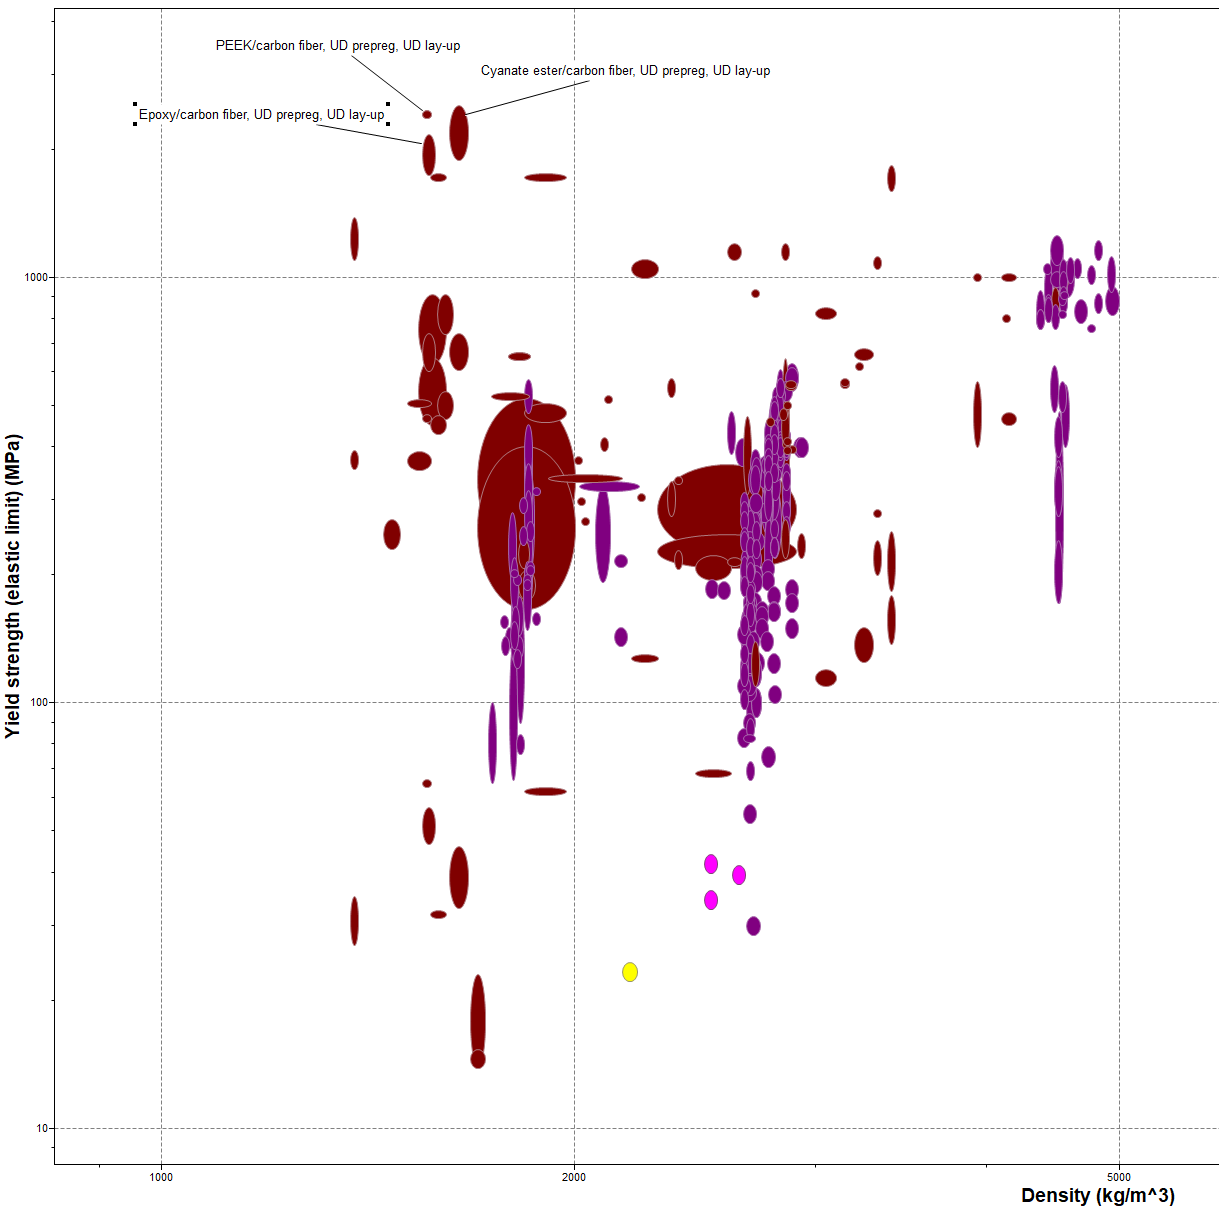
\includegraphics[width=.5\textwidth]{CESmatchoicebad}
    \caption{Cambridge Engineering Selector (CES) showing the various aerospace grade materials usable for this application. The dark red dots are compositites, while the dark purple dots are metals such as aluminium and magnesium.}
    \label{fig:CESmatchoice}
  \end{figure}

\section{Composites}

  The strength of composites come from the fiber.

  \subsection{Sandwich Structure}

    The bending stiffness for a simple sandwich panel

  \subsection{Wing Deflection}

\section{Final Design of Rear Wing}
  \fxnote{Presentation of CAD Drawings and method of how we will get to this result}
  \fxnote{Rendering}

<<<<<<< HEAD
  The two elements of the full scale wing will be bolted to the endplates at the optimal found angle of attack. The wing elements will have two metal brackets glued to the inside of the carbon fiber wings, the bracket will be have holes with M10 threads in which the endplates are bolted to secure the structure.

  \subsection{Topology Optimization}

  In order to minimise the weight of the metal bracket inserts topology optimizations where made using the build in function in \textit{Fusion 360}, in which all simulations are done in the cloud. Topology optimization tries to reduce the weight of the model by removing excess material while maintaining stiffness and strength of the model.
  The inserts were modeled from the wing profile and the location of the inner threads was chosen. The model was then meshed with a target cell size of $\SI{1.5}{\mili\metre}$, and the target weight reduction was set to $\SI{70}{\%}$, with a downforce load of $\SI{250}{\Newton}$ at the surface.

  \begin{figure}
    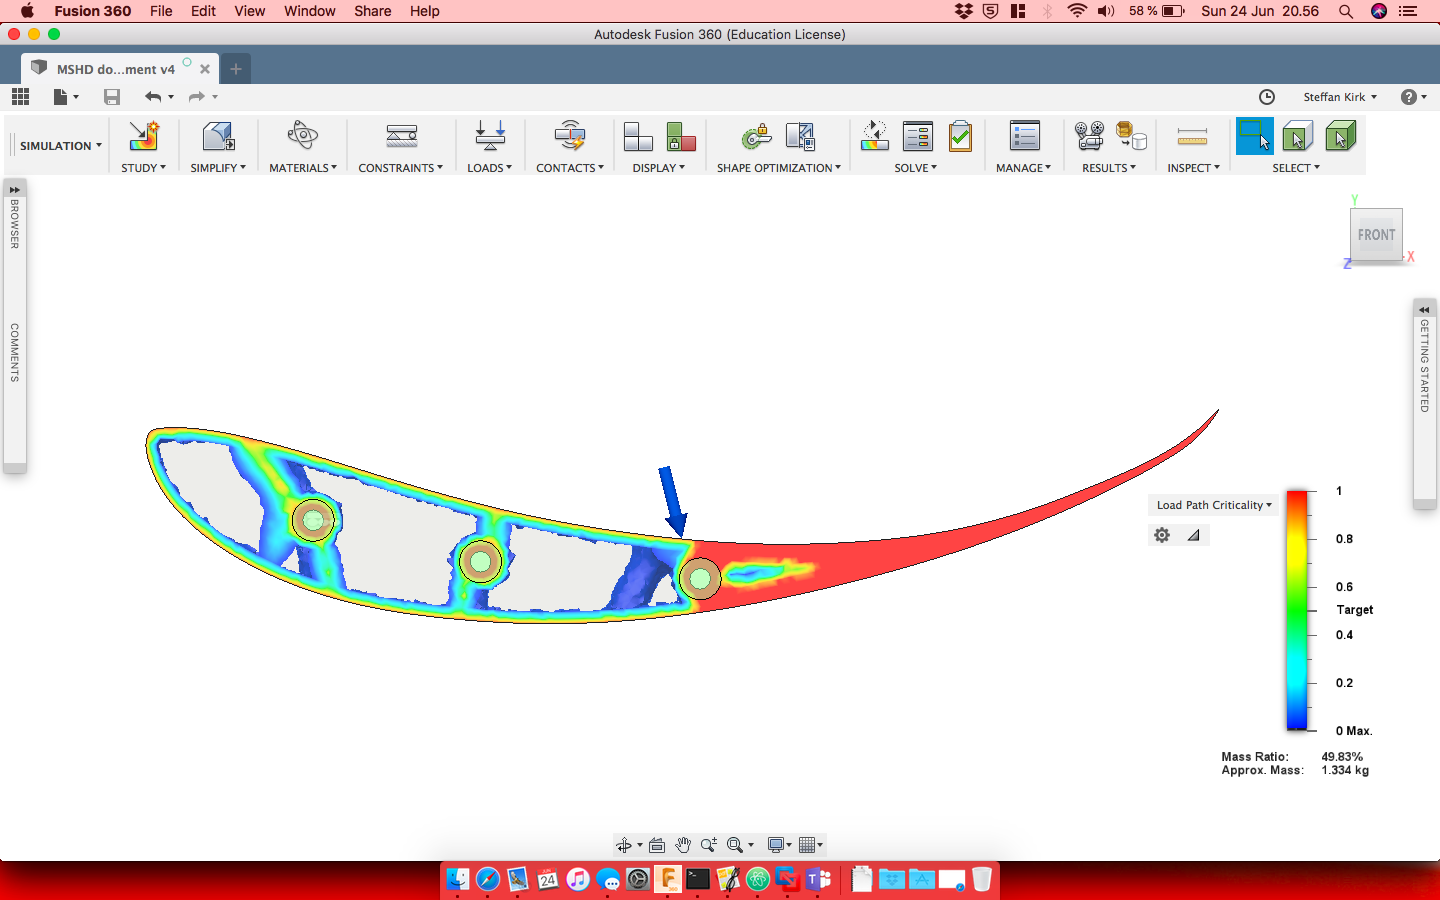
\includegraphics[width=\textwidth]{Optimisedlargewinginsert}
    \caption{The result of the topology optimization for the large insert, with a weight reduction at about $\SI{50}{\%}$.}
    \label{fig:topology_large_insert}
  \end{figure}

  The result of the optimization for the large insert is shown in figure \ref{fig:topology_large_insert}, was then used to remove excess material from the model. The results were overlayed on the model and material could be cut from the original model as shown in figure
  \ref{fig:meshoverlay}. The final model of the large insert was then created with a weight reduction around $\SI{40}{\%}$. A render of the final model is shown in
  figure \ref{fig:render_large_insert}.

  \begin{figure}
    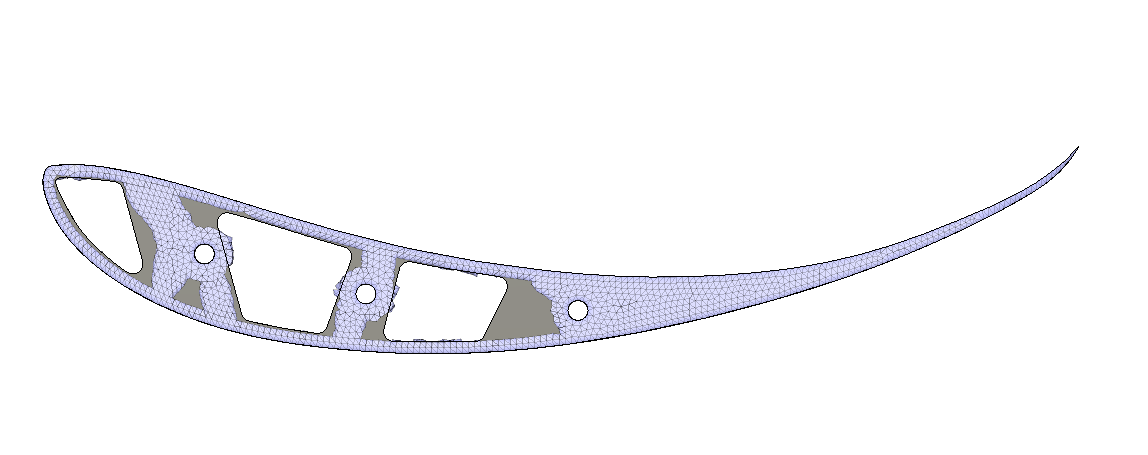
\includegraphics[width=\textwidth]{meshoverlayedlargeinsert}
    \caption{Optimized mesh overlayed on model so excess material could be easily removed.}
    \label{fig:meshoverlay}
  \end{figure}

  \begin{figure}
    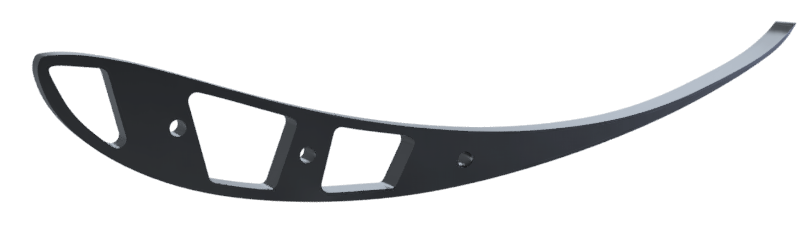
\includegraphics[width=\textwidth]{largeinsertrender}
    \caption{Render of the final model for the metal insert, with a weight reduction around $\SI{40}{\%}$.}
    \label{fig:render_large_insert}
  \end{figure}
=======
  The two elements of the full scale wing will be bolted to the end plates at optimal found angle of attack. The wing elements will have two metal brackets glued to the inside of the carbon fiber, the bracket will be have holes with M10 threads in which the endplates are bolted to secure the structure.

  \subsection{Topology Optimization}

  In order to minimise the weight of the metal bracket inserts topology optimizations where made using the build in function in \emph{Fusion 360}, where all simulations are done in the cloud.

>>>>>>> eddc32c69b3637929d7f9342c4da3fc5879469d6

  \subsection{Blue Prints}

\section{Manufacturing Final Design}
  \subsection{Polystyrene Molds}

  \begin{figure}
    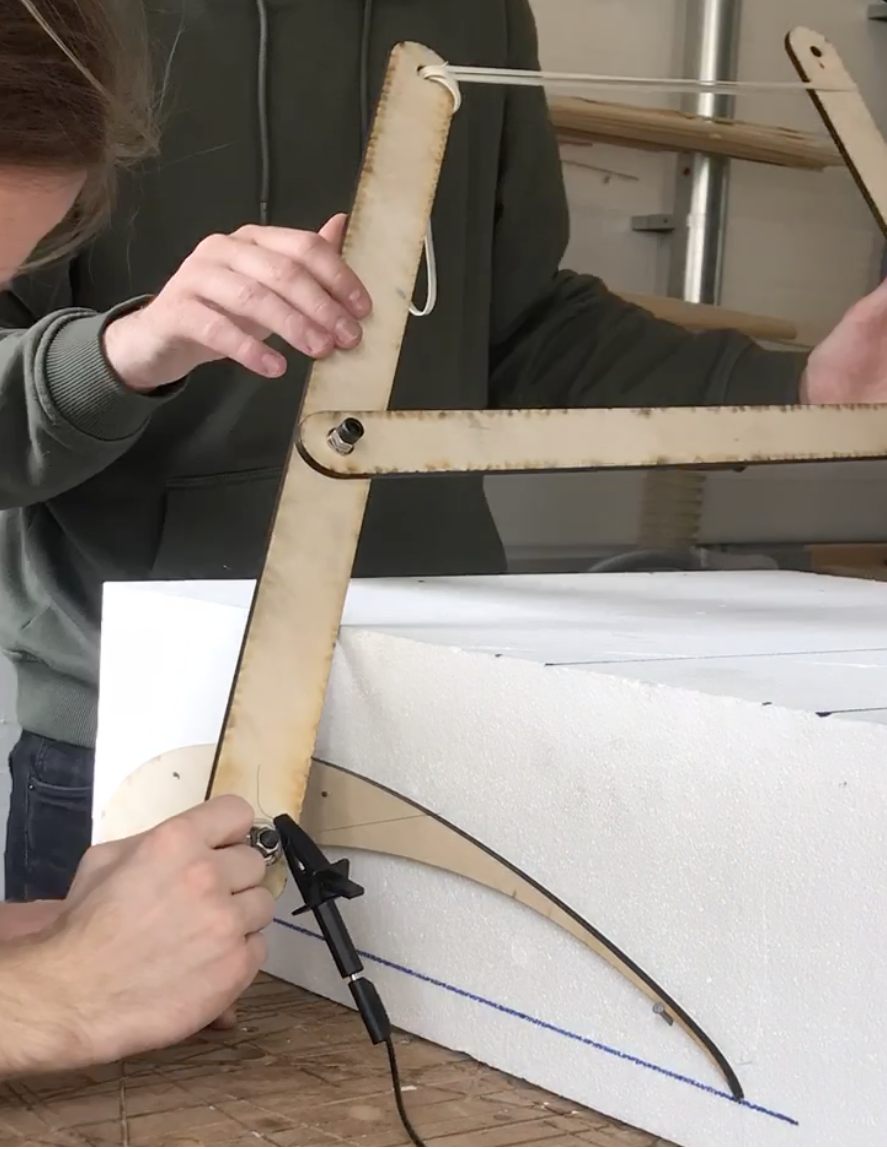
\includegraphics[width=\textwidth]{hotwiremethod}
    \caption{The hot wire melts the styrofoam while sliding along the wooden template.}
    \label{fig:hotwire}
  \end{figure}

  The molds for the wings were chosen as positive molds, meaning polystyrene molds of the actual wings were cut out and overlaid with resin coated carbon fiber. In order to do this, we devised a hotwire-based specialized tool for the job. This can be seen in figure \ref{fig:hotwire}, where a gauge 4 wire was used at $\SI{12}{\volt}$ drawing $\SI{2.5}{\ampere}$ over a cutting length of $\SI{600}{\milli\metre}$. In order to get the correct airfoil shapes, the MSHD airfoil profile was lasercut out of 3mm plywood. The wooden profile is then mounted on the sides of the polystyrene block, where the hotwire is pulled across in a timely fashion. In order to produce a smooth surface, two people have to move very coordinated. Going too slow leaves deep melting lines, and moving too fast lets the hotwire ''slack'' in the middle because it does not melt the polystyrene quick enough, which causes the airfoil profile to be skewed.

  All hotwire cutting was done by hand over several days, and we owe a special thanks to our sponsor DTU Skylab for providing the polystyrene blocks.



  \subsection{Hand Layup}
    \begin{figure}
      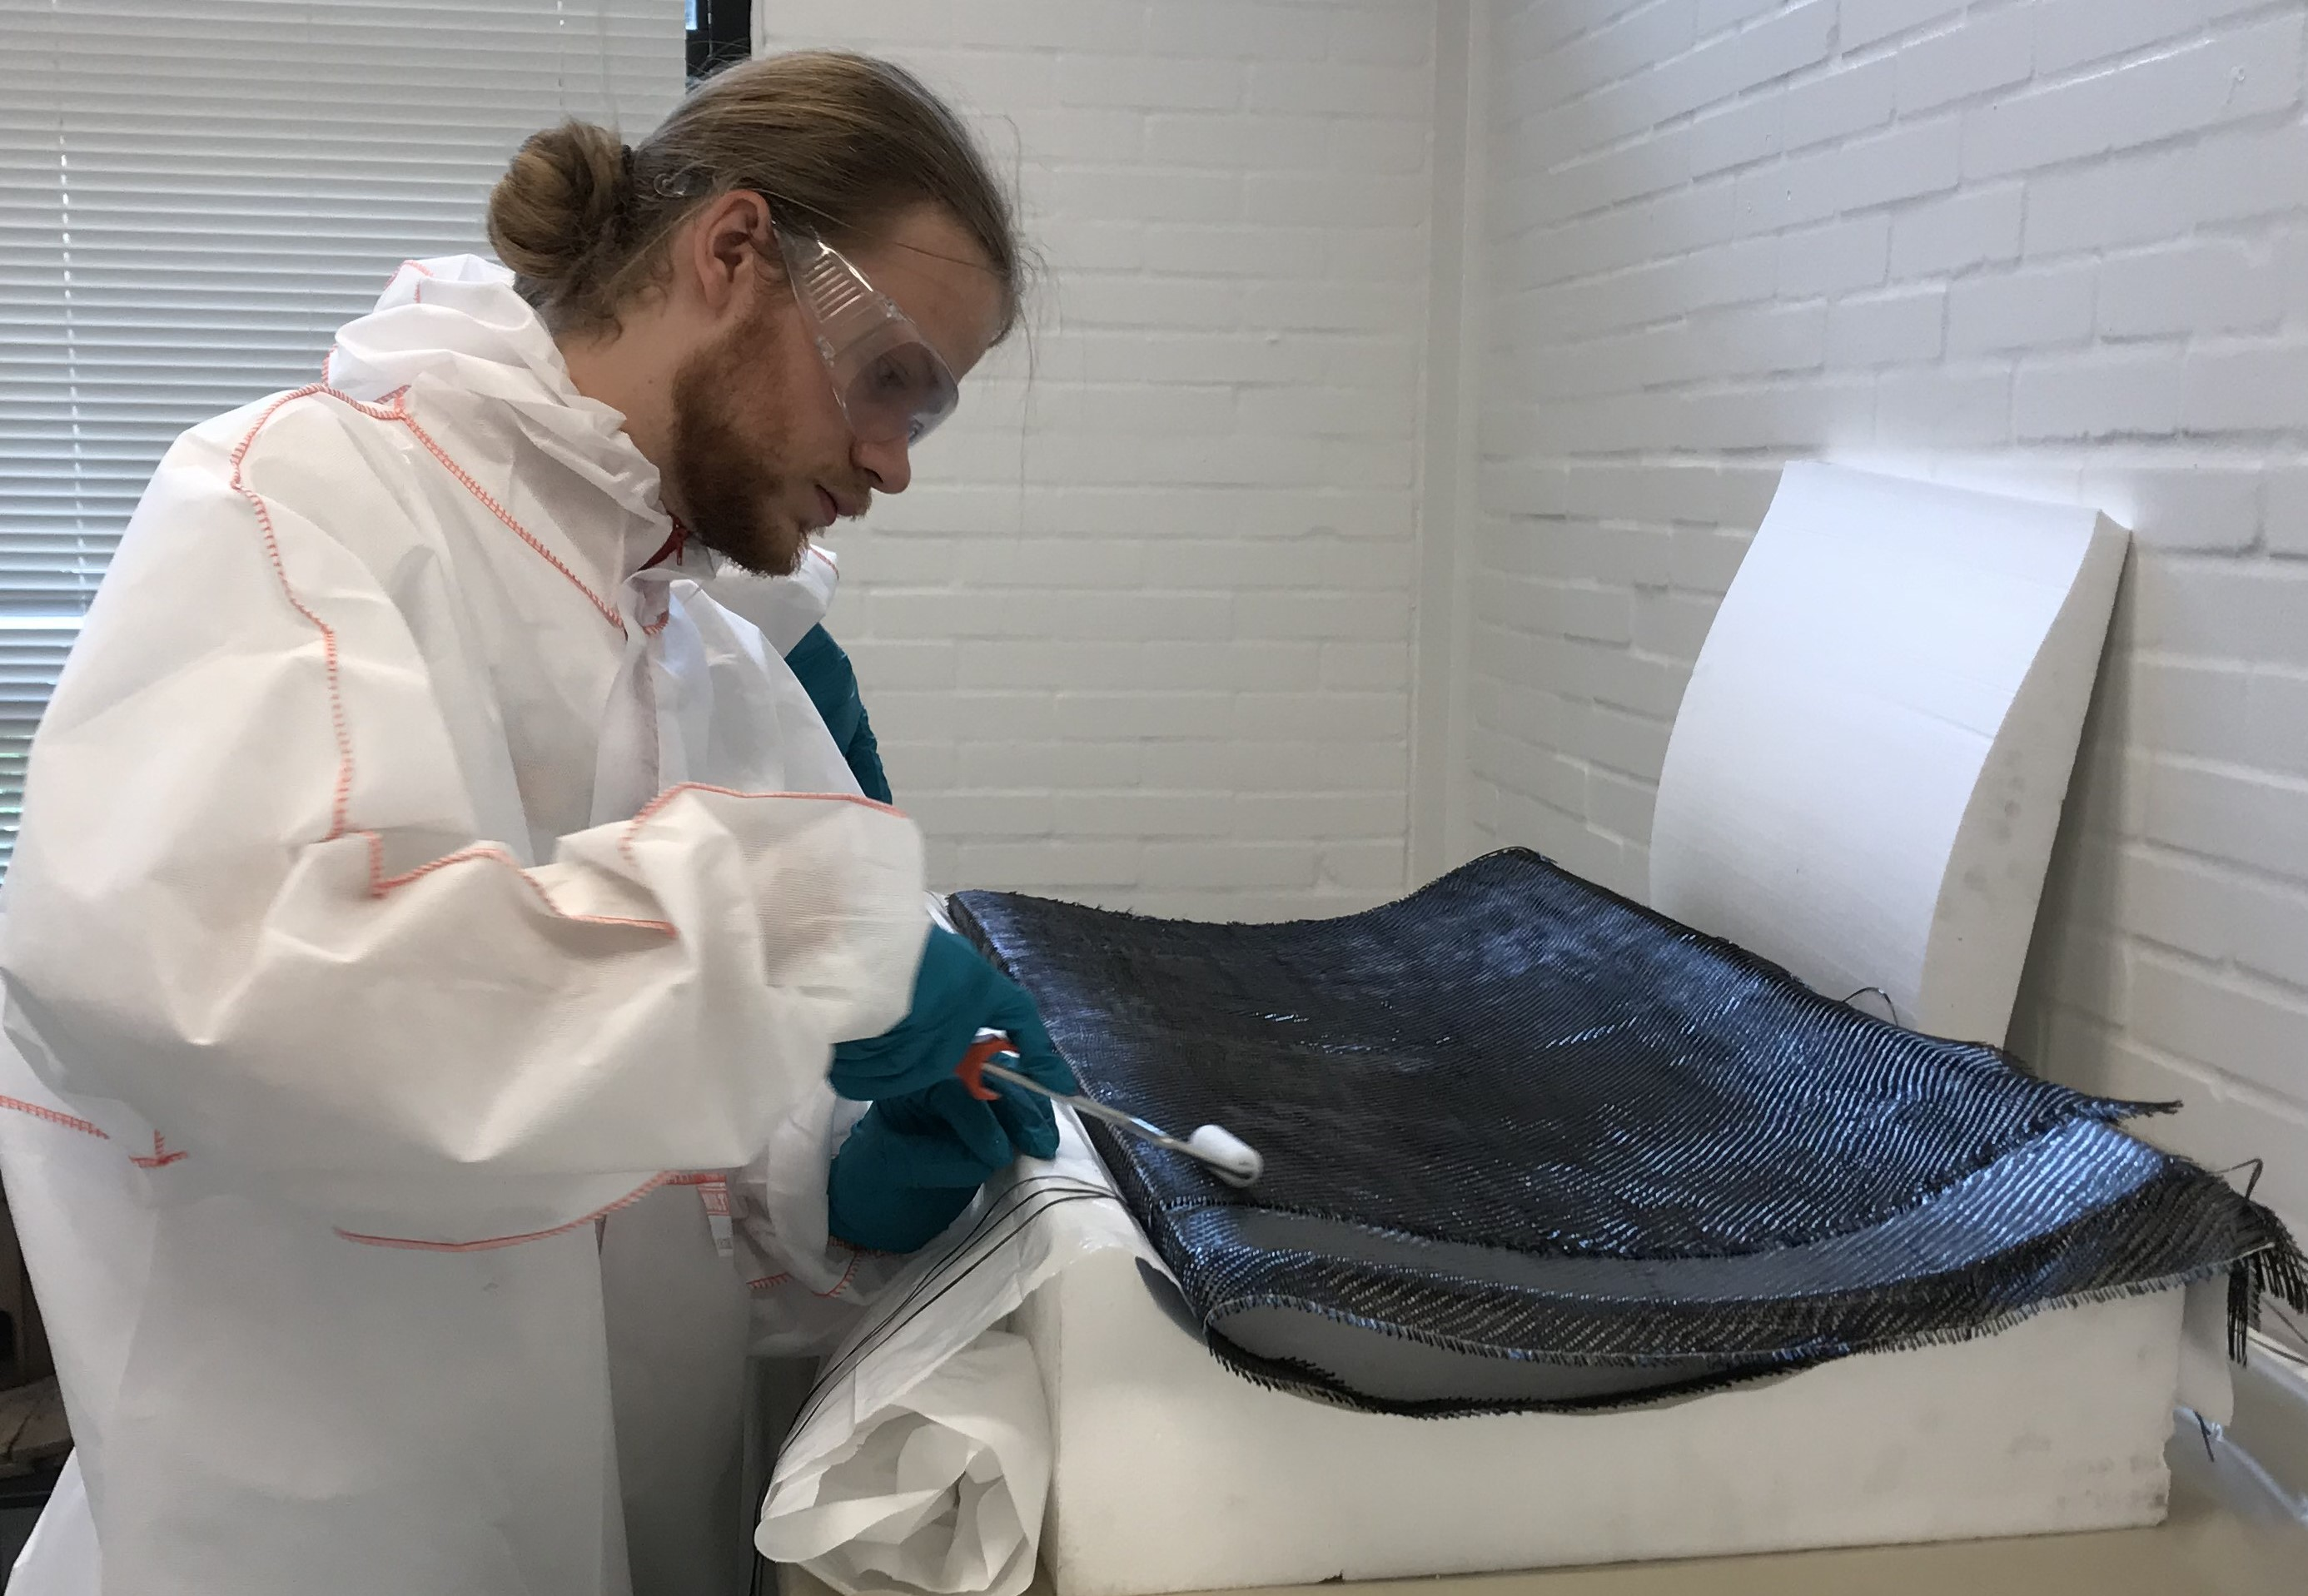
\includegraphics[width=\textwidth]{handlayupwnicolai}
      \caption{Steffan and Nicolai performing a hand layup of the carbon fiber mats around a polystyrene foam core.}
      \label{fig:handlayup}
    \end{figure}

    \fxnote{Show how we did the hand lay up. What went wrong what went well.}

  \subsection{Surface Finish}

    \begin{figure}
      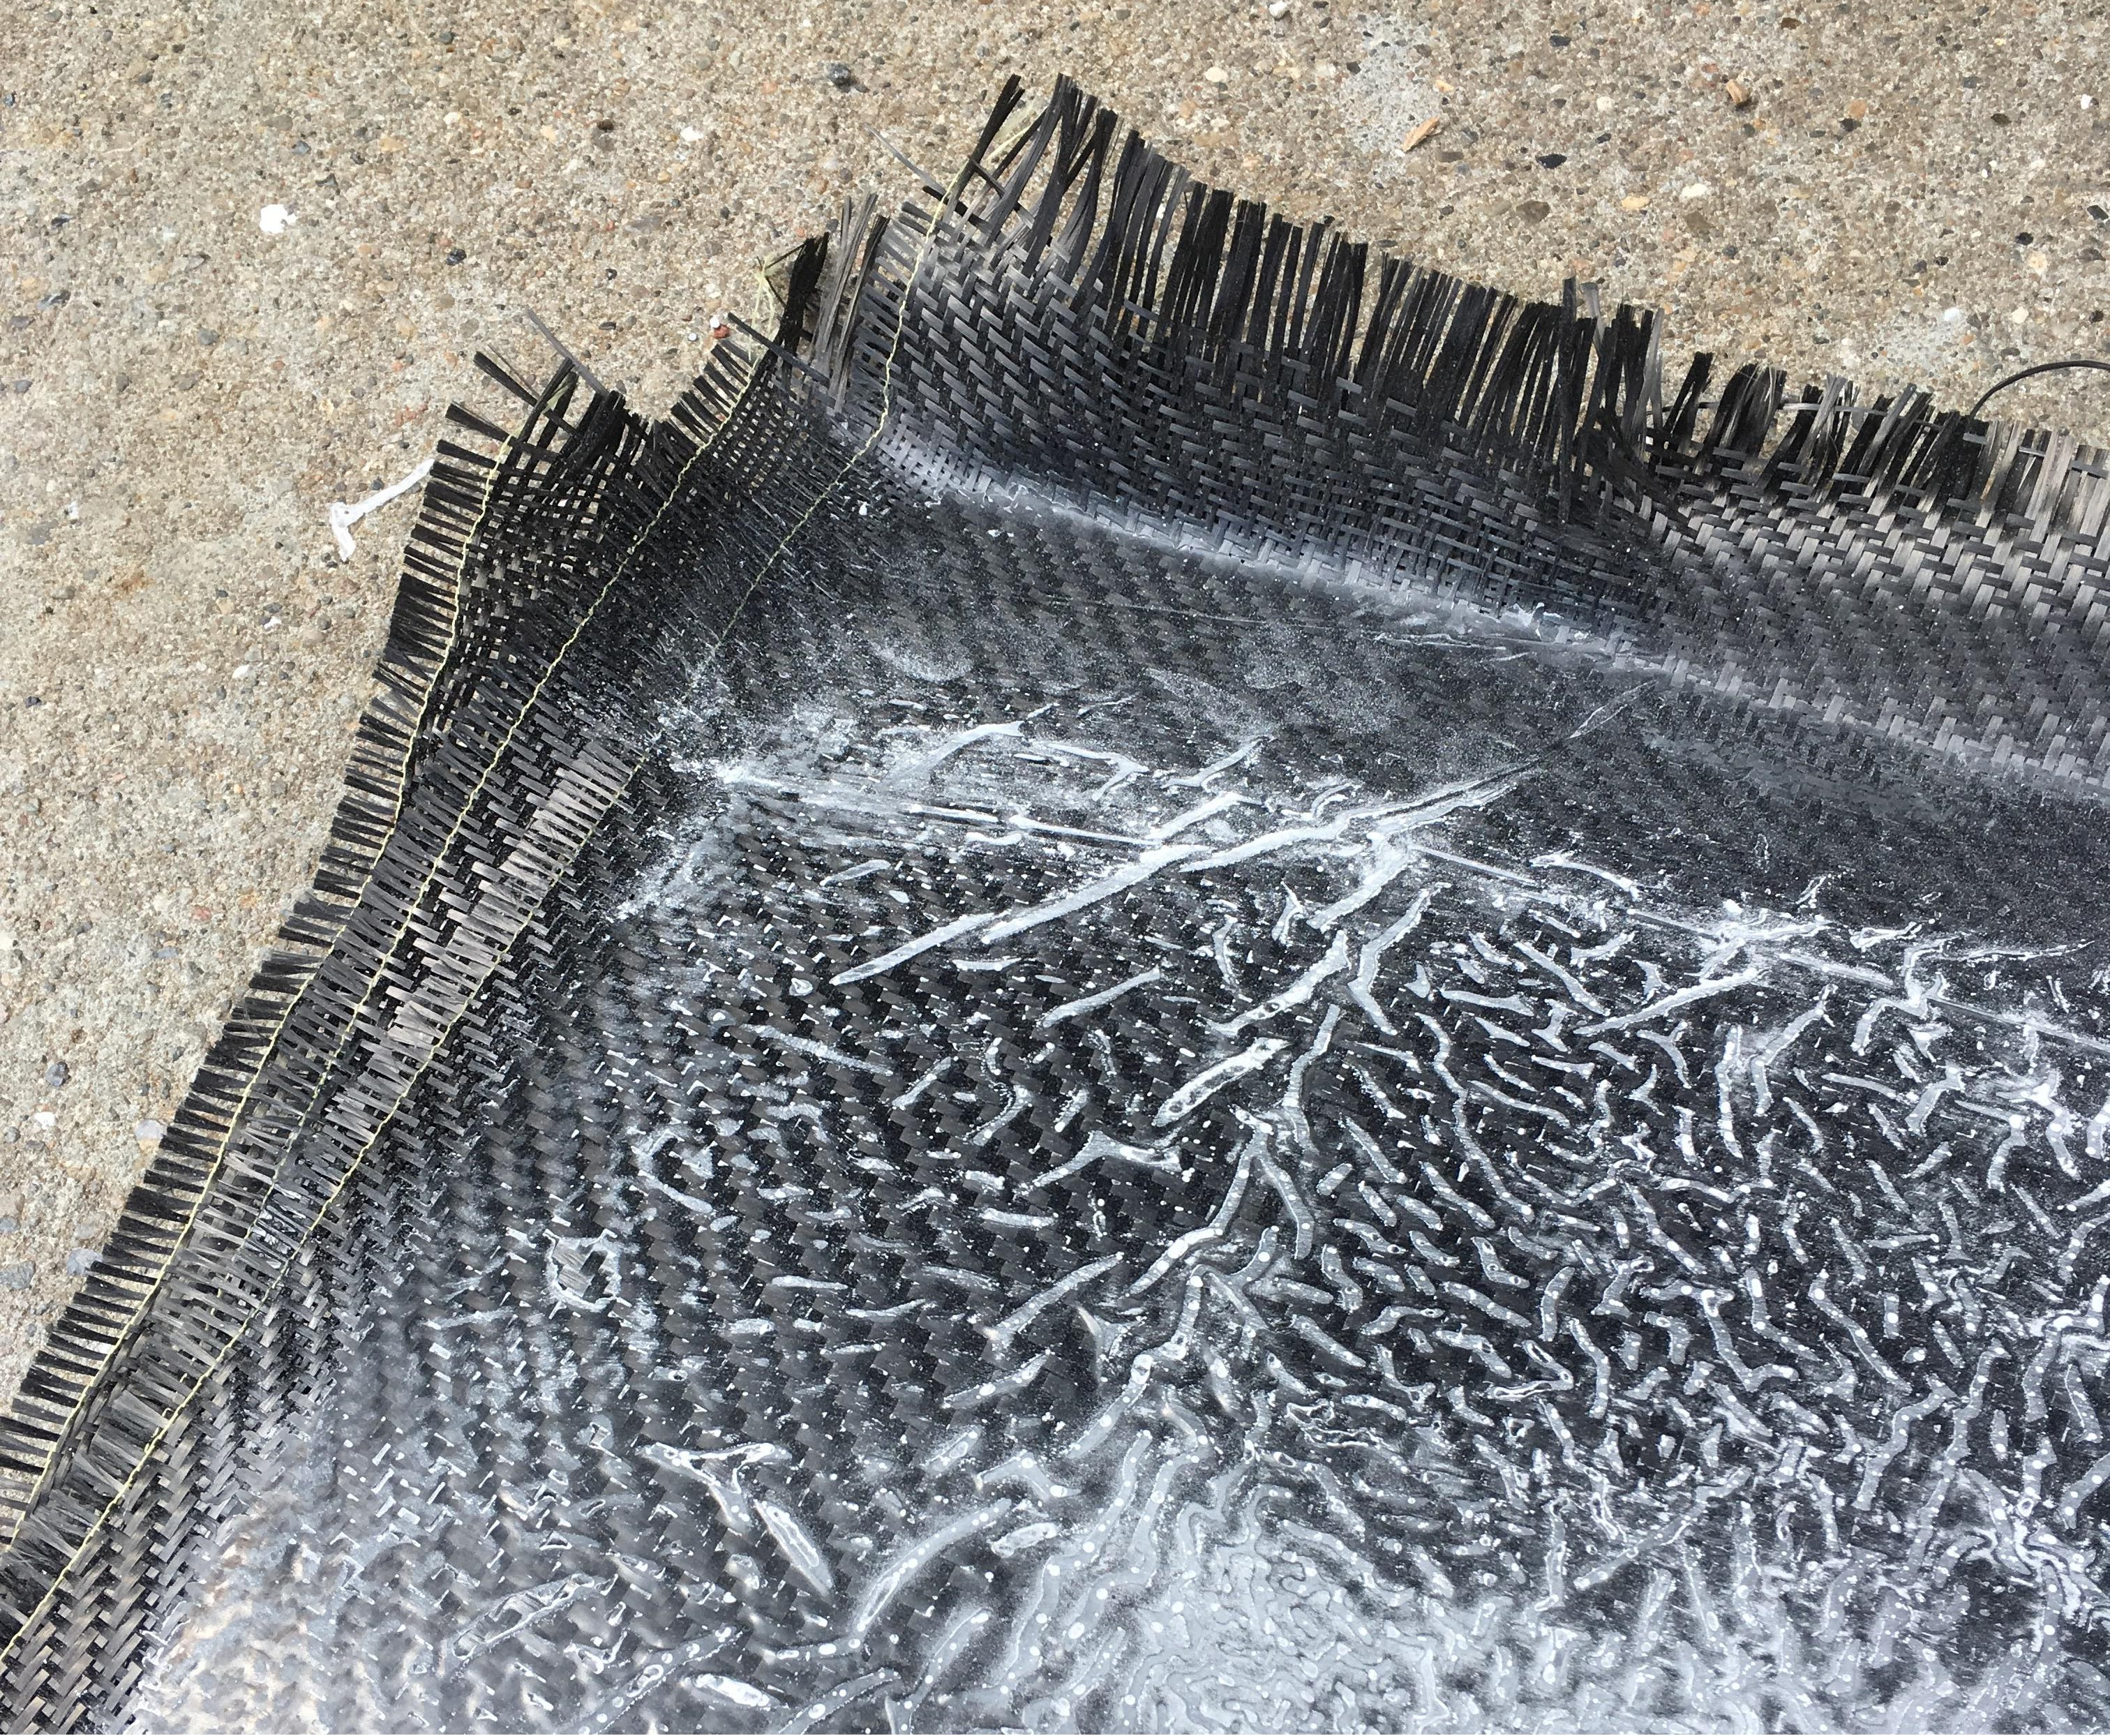
\includegraphics[width=\textwidth]{residualepoxy}
      \caption{Curing the wing in a flat position let the resin pool in the center of the wing, making the surface very rough.}
      \label{fig:roughsurface}
    \end{figure}

    \begin{figure}
      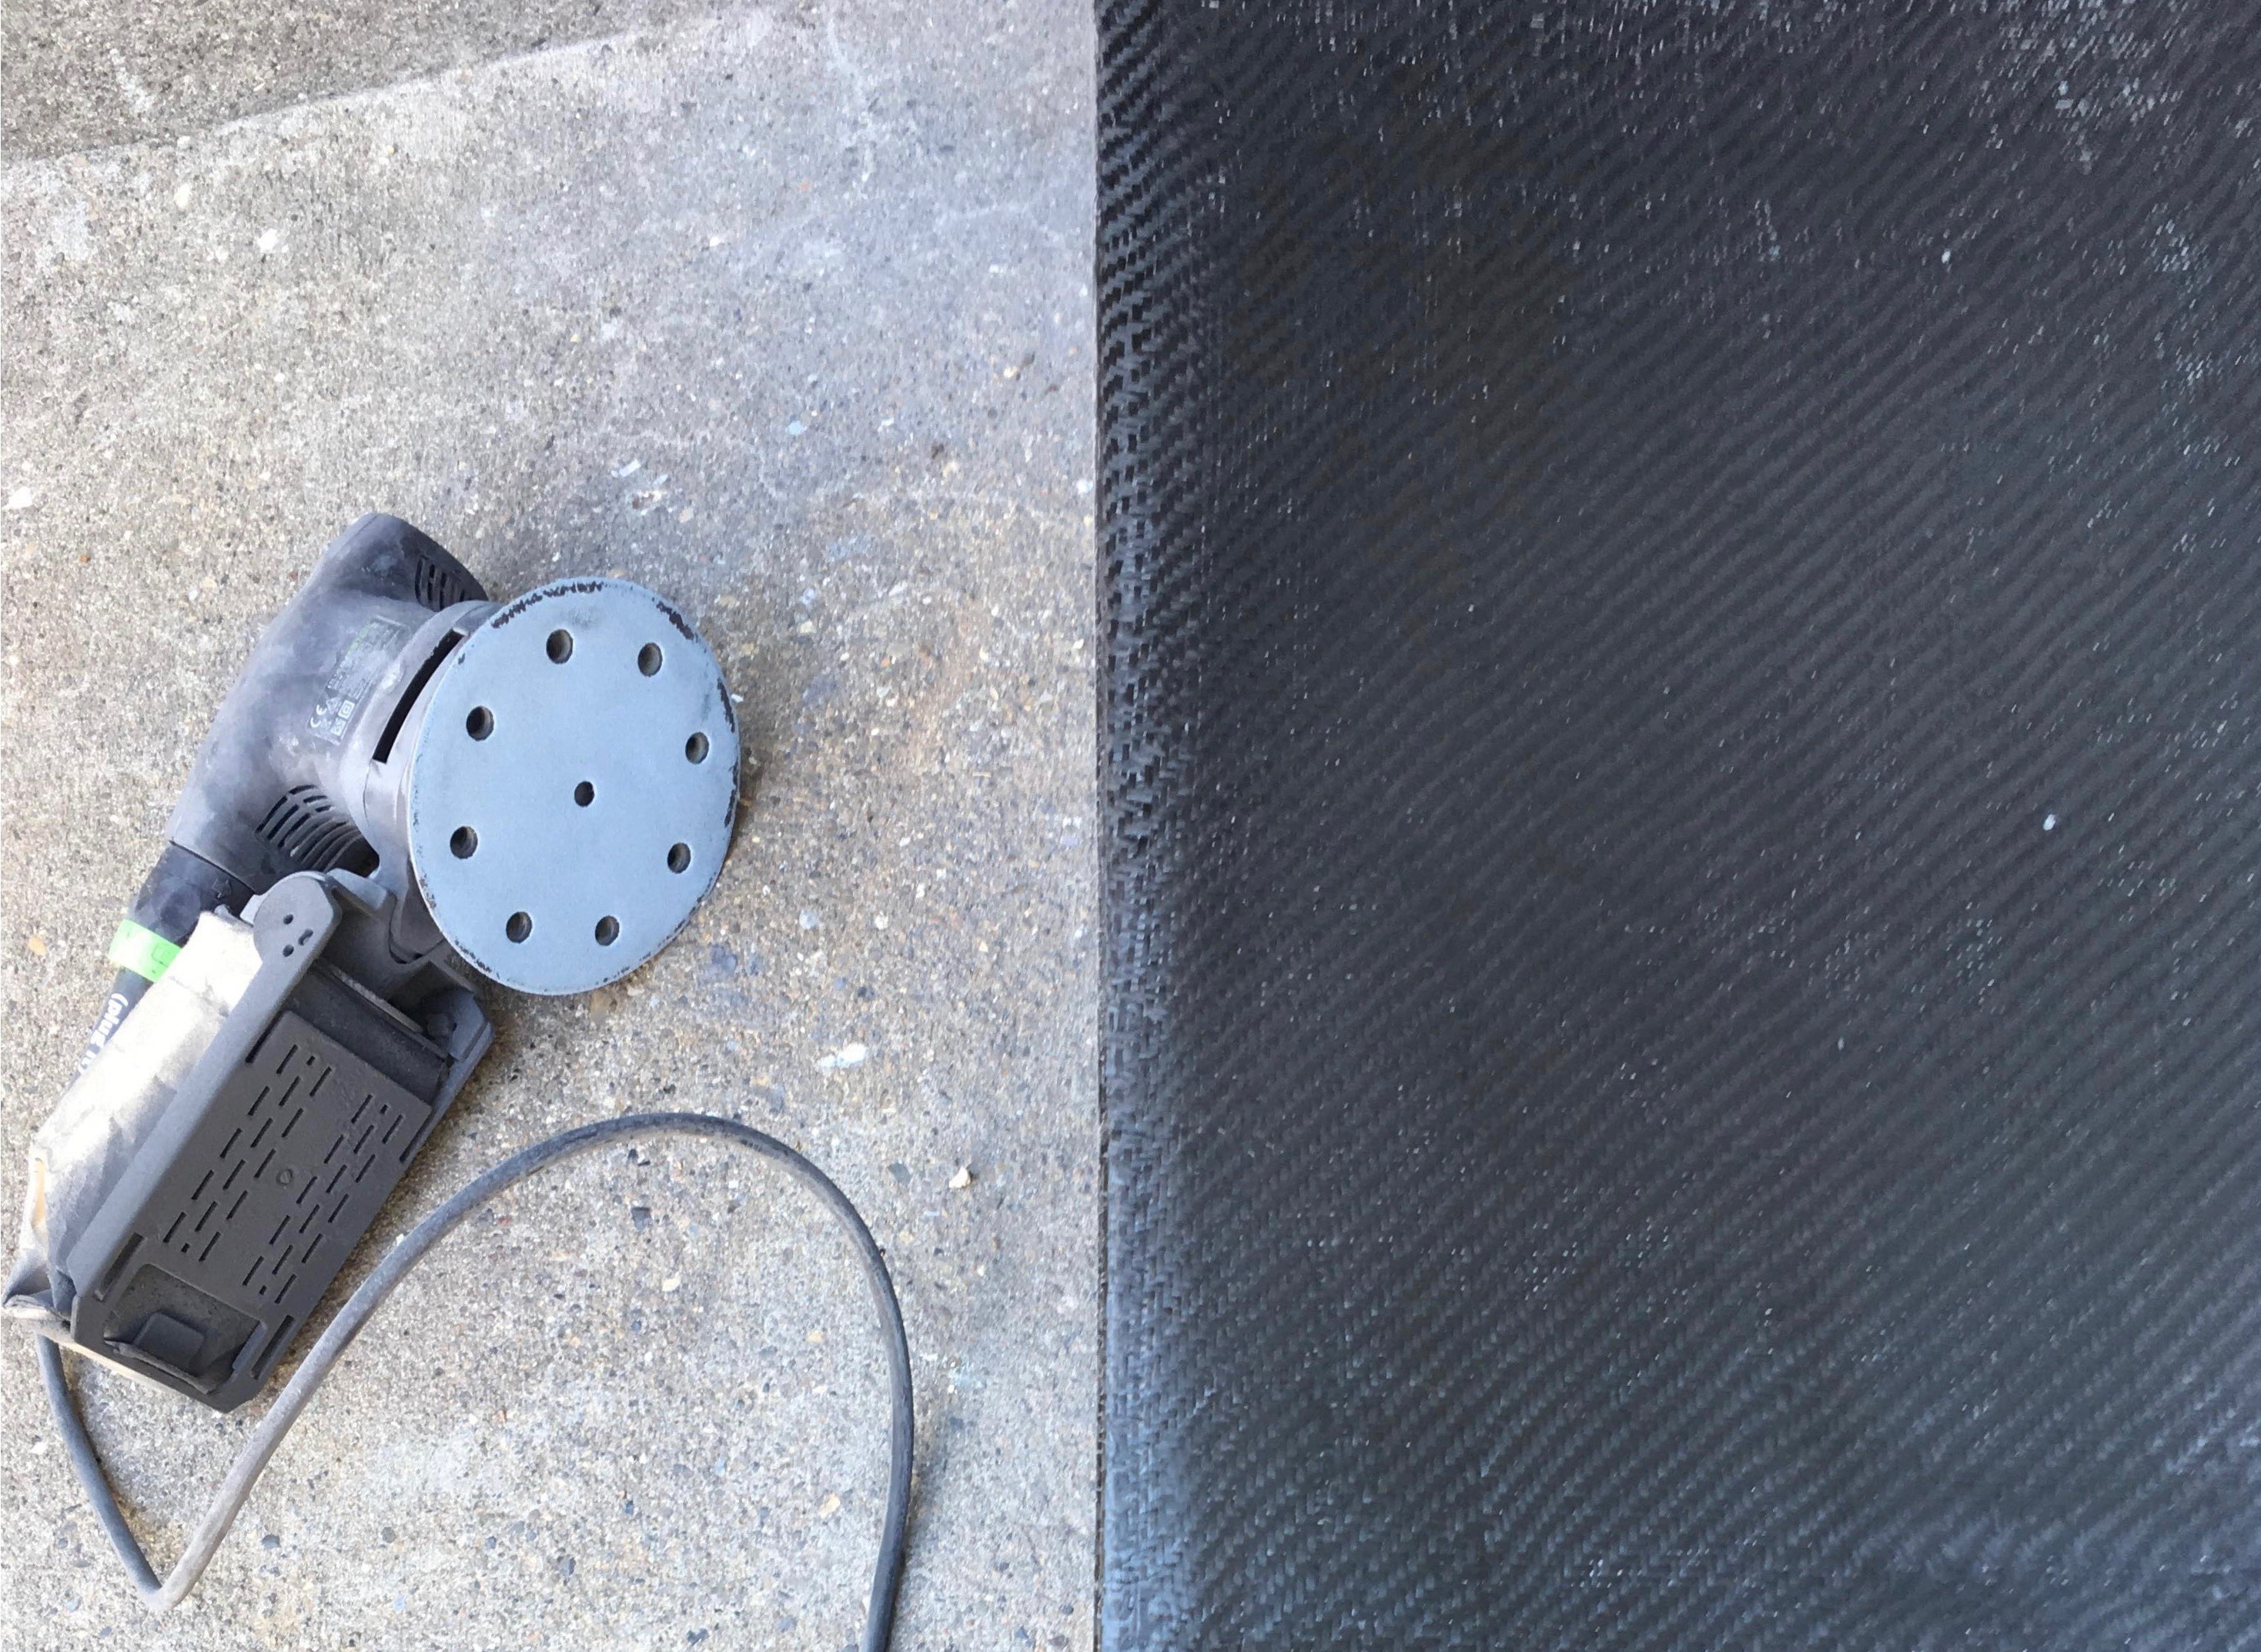
\includegraphics[width=\textwidth]{wingaftersandingperfect}
      \caption{Sanding the wing clears the surface roughness, but requires a new layer of sealant. Using epoxy or a lacquer was investigated before settling on epoxy.}
      \label{fig:wingaftersanding}
    \end{figure}

  \subsection{Implementation and Testing}

\section{Testing and Inspection}

  \subsection{Reinforcing the mounting}
